\documentclass[12pt,a4paper]{article}

\usepackage[utf8]{inputenc}
\usepackage[T1]{fontenc}
\usepackage[brazil]{babel}
\usepackage[margin=2.5cm]{geometry}
\usepackage{graphicx}
\usepackage{booktabs}
\usepackage{array}
\usepackage{multirow}
\usepackage{longtable}
\usepackage[table]{xcolor}
\usepackage{amsmath}
\usepackage{enumitem}
\usepackage{fancyhdr}
\usepackage{titlesec}
\usepackage{hyperref}
\usepackage{placeins}

\hypersetup{
  colorlinks=true,
  linkcolor=black,
  urlcolor=blue!60!black,
  citecolor=black
}

% Figuras: fotos locais + figuras reutilizadas do artigo
\graphicspath{{./}{../artigo/NILM2/figuras/}{../artigo/NILM/figuras/}}

% Cabeçalho institucional
\pagestyle{fancy}
\fancyhf{}
\fancyhead[L]{\footnotesize IFMT -- Campus Cuiab\'a Cel. Octayde Jorge da Silva}
\fancyhead[R]{\footnotesize Extens\~ao II -- 2026/1}
\fancyfoot[C]{\thepage}
\renewcommand{\headrulewidth}{0.4pt}

\titleformat{\section}{\Large\bfseries\color{green!35!black}}{\thesection}{0.6em}{}
\titleformat{\subsection}{\large\bfseries}{\thesubsection}{0.6em}{}

\setlength{\parskip}{0.6em}
\setlength{\parindent}{0pt}

\begin{document}

% ======================================================================
% CAPA
% ======================================================================
\begin{titlepage}
\centering
\vspace*{1cm}

{\Large\bfseries INSTITUTO FEDERAL DE MATO GROSSO}\\[0.2cm]
{\large Campus Cuiab\'a Coronel Octayde Jorge da Silva}\\[0.1cm]
{\normalsize Departamento de Computa\c{c}\~ao (DCOM)}\\[0.1cm]
{\normalsize Curso de Engenharia da Computa\c{c}\~ao}\\[2.5cm]

\rule{\linewidth}{0.4pt}\\[0.6cm]
{\LARGE\bfseries AccuEnergy: Medidor Bif\'asico de Energia com\\[0.2cm]
Monitoramento N\~ao Intrusivo de Cargas (NILM)\\[0.2cm]
em Arquitetura \textit{Edge-to-Server} de Baixo Custo}\\[0.6cm]
\rule{\linewidth}{0.4pt}\\[2.5cm]

{\large\bfseries Relat\'orio Final}\\[0.3cm]
{\normalsize Disciplina de Extens\~ao II}\\[0.1cm]
{\normalsize Professor: Tiago Lacerda}\\[3cm]

{\large \textbf{Autor:} Carlos Miguel Oliveira de Moraes e Silva}\\[0.2cm]
{\normalsize GitHub: \texttt{cmigos1}}\\[0.1cm]
{\normalsize Fun\c{c}\~ao: Desenvolvimento integral (\textit{firmware}, \textit{backend}, an\'alise de dados)}\\

\vfill
{\normalsize Cuiab\'a -- MT\\ 2026}
\end{titlepage}

\tableofcontents
\newpage

% ======================================================================
% 1. IDENTIFICAÇÃO
% ======================================================================
\section{Identifica\c{c}\~ao do Projeto}

\subsection{T\'itulo do Projeto}

\textbf{AccuEnergy} --- Medidor bif\'asico de energia el\'etrica com Monitoramento
N\~ao Intrusivo de Cargas (NILM, do ingl\^es \textit{Non-Intrusive Load
Monitoring}) implementado sobre uma arquitetura \textit{Edge-to-Server} de baixo
custo relativo, baseada nos microcontroladores STM32H743 e ESP32.

\subsection{Curso / Disciplina / Professor}

\begin{itemize}[nosep]
  \item \textbf{Curso:} Engenharia da Computa\c{c}\~ao
  \item \textbf{Disciplina:} Extens\~ao II -- Per\'iodo 2026/1
  \item \textbf{Professor respons\'avel:} Tiago Lacerda
  \item \textbf{Institui\c{c}\~ao:} IFMT -- Campus Cuiab\'a Cel. Octayde Jorge da Silva
\end{itemize}

\subsection{Integrantes}

O projeto foi desenvolvido de forma \textbf{individual}. O autor acumulou todas as
fun\c{c}\~oes t\'ecnicas ao longo do semestre:

\begin{longtable}{p{4.5cm} p{9.5cm}}
\toprule
\textbf{Integrante} & \textbf{Fun\c{c}\~oes desempenhadas} \\
\midrule
\endhead
Carlos Miguel Oliveira de Moraes e Silva \newline (GitHub: \texttt{cmigos1}) &
Concep\c{c}\~ao da arquitetura; desenvolvimento de \textit{firmware} embarcado
(STM32H743 e ESP32); projeto do condicionamento de sinais; \textit{backend} de
ingest\~ao (Python/MQTT); an\'alise de dados e desagrega\c{c}\~ao NILM; reda\c{c}\~ao
da documenta\c{c}\~ao t\'ecnica e do artigo. \\
\bottomrule
\end{longtable}

\subsection{Local e Ano}

Cuiab\'a -- MT, Instituto Federal de Mato Grosso (IFMT), Campus Cuiab\'a Cel.
Octayde Jorge da Silva, 2026.

% ======================================================================
% 2. RESUMO EXECUTIVO
% ======================================================================
\section{Resumo Executivo}

\textbf{Problema.} O monitoramento detalhado do consumo el\'etrico residencial
normalmente exige sensores dedicados por aparelho (monitoramento intrusivo), o que
implica alto custo e complexidade de instala\c{c}\~ao. Solu\c{c}\~oes de NILM,
que inferem o consumo individual a partir de um \'unico ponto de medi\c{c}\~ao,
costumam depender de \textit{hardware} de aquisi\c{c}\~ao caro.

\textbf{P\'ublico-alvo.} Consumidores residenciais interessados em efici\^encia
energ\'etica e a comunidade acad\^emica de sistemas embarcados e processamento de
sinais, que pode reaproveitar a plataforma aberta como base de estudo.

\textbf{Produto desenvolvido.} Um medidor bif\'asico de baixo custo relativo que
adquire tens\~ao e corrente em alta frequ\^encia (15{.}360~Hz por fase), calcula
grandezas el\'etricas e o espectro harm\^onico na borda, transmite as
caracter\'isticas via MQTT e realiza a desagrega\c{c}\~ao de cargas por
aprendizado de m\'aquina em um servidor dedicado. O sistema divide o
\textit{pipeline} entre um n\'o sensor embarcado (borda) e um servidor
(\textit{Edge-to-Server}).

\textbf{Tecnologias.} STM32H743 (aquisi\c{c}\~ao/DSP), ESP32 (Wi-Fi/MQTT),
sensores SCT-013 e ZMPT101B, \textit{broker} Mosquitto, Python (PyQt5,
\texttt{paho-mqtt}, \textit{pandas}, \textit{scikit-learn}), \textit{toolkit}
NILMTK.

\textbf{Principais resultados.} O sistema realiza aquisi\c{c}\~ao bif\'asica
simult\^anea est\'avel, calcula pot\^encia ativa/reativa/aparente, fator de
pot\^encia e Distor\c{c}\~ao Harm\^onica Total (DHT) sem \textit{jitter}, e mant\'em
um servidor de registro cont\'inuo resiliente. Na desagrega\c{c}\~ao, o agrupamento
n\~ao supervisionado identifica assinaturas das cargas de maior pot\^encia, mas a
resolu\c{c}\~ao fina se degrada com o ac\'umulo de eventos de baixa pot\^encia. Um
teste de nulidade demonstrou, como achado relevante, que as caracter\'isticas
harm\^onicas n\~ao agregam informa\c{c}\~ao discriminativa ao agrupamento no
cen\'ario avaliado.

% ======================================================================
% 3. VISÃO DO PROJETO
% ======================================================================
\section{Vis\~ao do Projeto}

\textbf{Descri\c{c}\~ao do problema.} Medir o consumo de cada eletrodom\'estico de
uma resid\^encia \'e valioso para incentivar a efici\^encia energ\'etica, mas
inviabiliza-se pela necessidade de um sensor por carga. O NILM resolve isso ao
desagregar o consumo total a partir de um \'unico ponto de medi\c{c}\~ao no quadro
de entrada; contudo, a literatura reporta forte depend\^encia de \textit{hardware}
de aquisi\c{c}\~ao de alto custo, o que limita a ado\c{c}\~ao em larga escala.

\textbf{P\'ublico-alvo e comunidade beneficiada.} Por se tratar de um projeto de
car\'ater t\'ecnico-experimental, sem parceiro externo formal, o p\'ublico-alvo
imediato \'e o consumidor residencial preocupado com efici\^encia energ\'etica.
Como benef\'icio secund\'ario, a plataforma --- integralmente documentada e
disponibilizada em reposit\'orio p\'ublico --- serve de refer\^encia aberta para
estudantes e pesquisadores de sistemas embarcados, instrumenta\c{c}\~ao eletr\^onica
e aprendizado de m\'aquina aplicado \`a energia.

\textbf{Justificativa.} Demonstrar que \'e poss\'ivel construir um n\'o de
medi\c{c}\~ao NILM com fidelidade adequada usando componentes de baixo custo
relativo tem impacto direto na democratiza\c{c}\~ao do monitoramento energ\'etico.
A engenharia de caracter\'isticas na borda reduz o tr\'afego de dados de megabytes
para poucos kilobytes por segundo, viabilizando a opera\c{c}\~ao cont\'inua.

\textbf{Objetivos.}
\begin{itemize}[nosep]
  \item \textbf{Geral:} projetar e validar um medidor bif\'asico NILM de baixo
  custo sob o paradigma \textit{Edge-to-Server}.
  \item \textbf{Espec\'ificos:} (i)~garantir aquisi\c{c}\~ao de alta fidelidade sem
  \textit{jitter}; (ii)~calcular grandezas el\'etricas e harm\^onicas na borda;
  (iii)~transmitir e persistir os dados de forma resiliente via MQTT;
  (iv)~aplicar detec\c{c}\~ao de eventos e agrupamento para desagregar cargas;
  (v)~avaliar criticamente a contribui\c{c}\~ao das caracter\'isticas harm\^onicas.
\end{itemize}

\textbf{Benef\'icios esperados.} Uma refer\^encia reprodut\'ivel de medidor NILM
acess\'ivel, com documenta\c{c}\~ao t\'ecnica completa, apta a ser estendida em
trabalhos futuros (protocolos de aquisi\c{c}\~ao estruturados, captura de
transit\'orios de \textit{inrush}, entre outros).

% ======================================================================
% 4. ROADMAP DO PRODUTO
% ======================================================================
\section{Roadmap do Produto}

O desenvolvimento foi organizado em \textbf{quatro \'epicos}, desdobrados em doze
hist\'orias de usu\'ario (\textit{user stories}) e distribu\'idos em tr\^es sprints
mensais (abril a junho de 2026). O \textit{Product Backlog} foi mantido em planilha
e o versionamento de c\'odigo no GitHub. A
Tabela~\ref{tab:backlog} apresenta o backlog priorizado; a coluna \textbf{Estado}
reflete a situa\c{c}\~ao ao fim do projeto.

\begin{longtable}{c p{5.6cm} c c c}
\caption{\textit{Product Backlog} priorizado, distribu\'ido por \'epico e sprint.}
\label{tab:backlog}\\
\toprule
\textbf{Hist.} & \textbf{Hist\'oria de usu\'ario} & \textbf{Prio.} & \textbf{Sprint} & \textbf{Estado} \\
\midrule
\endfirsthead
\multicolumn{5}{l}{\footnotesize\itshape continua\c{c}\~ao da Tabela~\ref{tab:backlog}}\\
\toprule
\textbf{Hist.} & \textbf{Hist\'oria de usu\'ario} & \textbf{Prio.} & \textbf{Sprint} & \textbf{Estado} \\
\midrule
\endhead
\multicolumn{5}{l}{\cellcolor{green!8}\textbf{EP1 -- Prototipagem de embarcado}} \\
US1 & Defini\c{c}\~ao de sensores e componentes passivos & M\'edia & 1 & Feito \\
US2 & \textit{Firmware} de amostragem (Vrms, Irms, Pot\^encia) & Alta & 1 & Feito \\
US3 & Montagem de prot\'otipo (adaptador SCT-013) & M\'edia & 1 & Feito \\
\midrule
\multicolumn{5}{l}{\cellcolor{green!8}\textbf{EP2 -- Calibra\c{c}\~ao e Tratamento}} \\
US4 & Calibra\c{c}\~ao de sensores e corre\c{c}\~ao de fase & Alta & 1 & Feito \\
US5 & Tratamento de ru\'ido (\textit{burst} + m\'edia m\'ovel) & Alta & 1 & Feito \\
\midrule
\multicolumn{5}{l}{\cellcolor{green!8}\textbf{EP4 -- Transmiss\~ao e \textit{Dataset}}} \\
US9  & Telemetria MQTT (\textit{task} de rede, JSON) & Alta & 2 & Feito \\
US10 & \textit{Backend} de ingest\~ao (\textit{broker} + \texttt{paho-mqtt}) & Alta & 2 & Feito \\
US11 & Tratamento de dados (CSV sequencial) & M\'edia & 2 & Feito \\
US12 & Persist\^encia local (kWh em LittleFS) & Baixa & 2 & Feito \\
\midrule
\multicolumn{5}{l}{\cellcolor{green!8}\textbf{EP3 -- Classifica\c{c}\~ao e Desagrega\c{c}\~ao} \footnotesize(\'unico \'epico incompleto)} \\
US6 & Curadoria de \textit{dataset} local rotulado & Alta & 3 & N\~ao conclu\'ido \\
US7 & Modelagem de classifica\c{c}\~ao (\textit{feature eng.}) & Alta & 3 & Substitu\'ido$^{*}$ \\
US8 & Estima\c{c}\~ao de consumo (infer\^encia cont\'inua) & Baixa & 3 & N\~ao conclu\'ido \\
\bottomrule
\end{longtable}

\noindent{\footnotesize $^{*}$ Substitu\'ido pela desagrega\c{c}\~ao \textbf{n\~ao
supervisionada} (detec\c{c}\~ao de eventos + K-means + teste de nulidade), efetivamente
entregue --- ver Se\c{c}\~ao~\ref{sec:resultados}.}

\textbf{Situa\c{c}\~ao de conclus\~ao.} Das doze hist\'orias planejadas, \textbf{nove
foram conclu\'idas} (\'epicos EP1, EP2 e EP4 integralmente). Apenas o \'epico EP3
--- \textbf{classifica\c{c}\~ao supervisionada} --- permaneceu incompleto: a
curadoria de \textit{dataset} rotulado (US6) e a estima\c{c}\~ao de consumo por
infer\^encia (US8) n\~ao foram finalizadas, enquanto a modelagem (US7) foi
substitu\'ida pela abordagem n\~ao supervisionada.

\textbf{Altera\c{c}\~oes durante o desenvolvimento.} O planejamento sofreu dois
desvios relevantes, ambos justificados:

\begin{enumerate}[nosep]
  \item \textbf{Pivot de \textit{hardware} (EP1/EP2).} A concep\c{c}\~ao original
  previa aquisi\c{c}\~ao \textbf{exclusivamente no ESP32}, via ADC nativo (US1--US5
  referem-se ao ADC1 do ESP32). Ao constatar-se que as interrup\c{c}\~oes da pilha
  Wi-Fi introduziam \textit{jitter} severo na amostragem, a arquitetura foi
  \textbf{redefinida} para um modelo h\'ibrido: STM32H743 dedicado \`a aquisi\c{c}\~ao
  e ESP32 dedicado \`a comunica\c{c}\~ao.
  \item \textbf{Permuta de EP3 e EP4.} O plano original alocava a
  desagrega\c{c}\~ao (EP3) na Sprint~2 e a transmiss\~ao/\textit{dataset} (EP4) na
  Sprint~3. Na pr\'atica, a ordem foi \textbf{invertida}: como a desagrega\c{c}\~ao
  depende do conjunto de dados produzido pela telemetria, o EP4 foi antecipado para
  a Sprint~2 e o EP3 realizado na Sprint~3.
  \item \textbf{Repriorização da desagrega\c{c}\~ao (EP3).} A classifica\c{c}\~ao
  supervisionada dependia de um \textit{dataset} rotulado (US6), invi\'avel de
  curar em ambiente residencial n\~ao controlado. O \'epico foi \textbf{reorientado}
  para desagrega\c{c}\~ao \textbf{n\~ao supervisionada} (detec\c{c}\~ao de eventos +
  K-means) acrescida de um teste de nulidade das caracter\'isticas harm\^onicas ---
  resultados efetivamente entregues (Se\c{c}\~ao~\ref{sec:resultados}).
\end{enumerate}

% ======================================================================
% 5. GESTÃO E TECNOLOGIAS
% ======================================================================
\section{Gest\~ao e Tecnologias}

\subsection{Gest\~ao do Projeto}

\begin{itemize}[nosep]
  \item \textbf{Metodologia:} Scrum adaptado ao contexto de projeto individual.
  O trabalho foi dividido em incrementos (sprints) com objetivo definido, revis\~ao
  ao final e replanejamento do \textit{backlog}.
  \item \textbf{Dura\c{c}\~ao das sprints:} sprints mensais (aproximadamente 4
  semanas cada).
  \item \textbf{Quantidade de sprints:} 3 sprints, de \textbf{abril a junho de
  2026} (Sprint~1 -- abril; Sprint~2 -- maio; Sprint~3 -- junho).
  \item \textbf{Ferramenta de gest\~ao:} planejamento e acompanhamento do
  \textit{Product Backlog} em \textbf{planilha Excel},
  versionamento e hist\'orico de entregas no \textbf{GitHub} (24 \textit{commits}).
  \item \textbf{Organiza\c{c}\~ao das tarefas:} cada sprint concentrou um conjunto
  de \'epicos; as entregas foram registradas como \textit{commits} descritivos,
  servindo de rastro de auditoria da evolu\c{c}\~ao.
  \item \textbf{Comunica\c{c}\~ao:} por ser projeto individual, a comunica\c{c}\~ao
  externa restringiu-se \`a orienta\c{c}\~ao docente e \`as revis\~oes de sprint.
\end{itemize}

\subsection{Tecnologias Utilizadas}

\begin{longtable}{p{5cm} p{9cm}}
\toprule
\textbf{Tecnologia} & \textbf{Finalidade} \\
\midrule
\endhead
STM32H743 (WeAct) & Aquisi\c{c}\~ao ADC/DMA de alta fidelidade e c\'alculo das grandezas el\'etricas \\
STM32CubeIDE / Linguagem C & Desenvolvimento do \textit{firmware} de aquisi\c{c}\~ao \\
ESP32 & N\'o de conectividade Wi-Fi/MQTT e ponte serial (\textit{bridge}) \\
PlatformIO / C++ (Arduino) & Desenvolvimento do \textit{firmware} do ESP32 \\
Sensor SCT-013-100 & Transformador de corrente n\~ao invasivo (n\'ucleo dividido) \\
Sensor ZMPT101B & Transdutor de tens\~ao isolado (\textit{standalone}) \\
Display ST7735 (SPI) & Indica\c{c}\~ao local de grandezas e status de calibra\c{c}\~ao \\
UART (460.800 \textit{baud}) & Barramento STM32 $\rightarrow$ ESP32 (\textit{frames} bin\'arios) \\
MQTT / Mosquitto & Protocolo e \textit{broker} de telemetria (servidor dedicado) \\
Python 3 / PyQt5 / pyqtgraph & Monitor de visualiza\c{c}\~ao em tempo real \\
\texttt{paho-mqtt} & Assinante MQTT e \textit{logger} para CSV \\
\textit{pandas}, \textit{numpy}, \textit{scikit-learn}, \textit{matplotlib} & An\'alise de dados, K-means e gera\c{c}\~ao de figuras \\
NILMTK (\textit{fork} local) & Detec\c{c}\~ao de eventos (Hart85) e valida\c{c}\~ao cruzada da desagrega\c{c}\~ao \\
Windows Task Scheduler & Persist\^encia dos servi\c{c}os (\textit{broker} e \textit{logger}) \\
Git / GitHub & Versionamento de c\'odigo e hist\'orico de \textit{commits}\\
\bottomrule
\end{longtable}

% ======================================================================
% 6. DESCRIÇÃO DO DESENVOLVIMENTO
% ======================================================================
\section{Descri\c{c}\~ao do Desenvolvimento}

A evolu\c{c}\~ao do projeto \'e descrita nas tr\^es sprints mensais. As entregas
correspondem aos marcos registrados no hist\'orico de \textit{commits} do
reposit\'orio e s\~ao ilustradas por fotografias do prot\'otipo.

\subsection{Sprint 1 -- Prototipagem e Calibra\c{c}\~ao (abril/2026)}
\begin{itemize}[nosep]
  \item \textbf{Objetivo:} prototipar o n\'o de medi\c{c}\~ao embarcado e calibrar
  o sensoriamento (\'epicos EP1 e EP2).
  \item \textbf{Planejado:} defini\c{c}\~ao de sensores e componentes passivos
  (US1), \textit{firmware} de amostragem (US2), montagem de prot\'otipo (US3),
  calibra\c{c}\~ao com corre\c{c}\~ao de fase (US4) e tratamento de ru\'ido (US5).
  \item \textbf{Conclu\'ido:} prot\'otipo em \textit{protoboard} com adaptador para
  o SCT-013; \textit{firmware} de amostragem AC com c\'alculo de $V_{rms}$,
  $I_{rms}$ e pot\^encia; calibra\c{c}\~ao contra mult\'imetro e filtro de m\'edia
  m\'ovel; teste inicial em uma \'unica fase (Figuras~\ref{fig:testeumafase}
  e~\ref{fig:prototipo}).
  \item \textbf{Dificuldade:} o \textit{jitter} induzido pela pilha Wi-Fi do ESP32
  comprometeu a estabilidade temporal da amostragem via ADC nativo.
  \item \textbf{Decis\~ao relevante:} \textbf{migrar a aquisi\c{c}\~ao para o
  STM32H743}, reservando o ESP32 para comunica\c{c}\~ao --- origem da arquitetura
  h\'ibrida. Ado\c{c}\~ao do ZMPT101B em modo \textit{standalone} (condicionamento
  passivo customizado).
  \item \textbf{Entrega:} prot\'otipo funcional monof\'asico calibrado.
\end{itemize}

\begin{figure}[ht]
  \centering
  \begin{minipage}{0.47\linewidth}
    \centering
    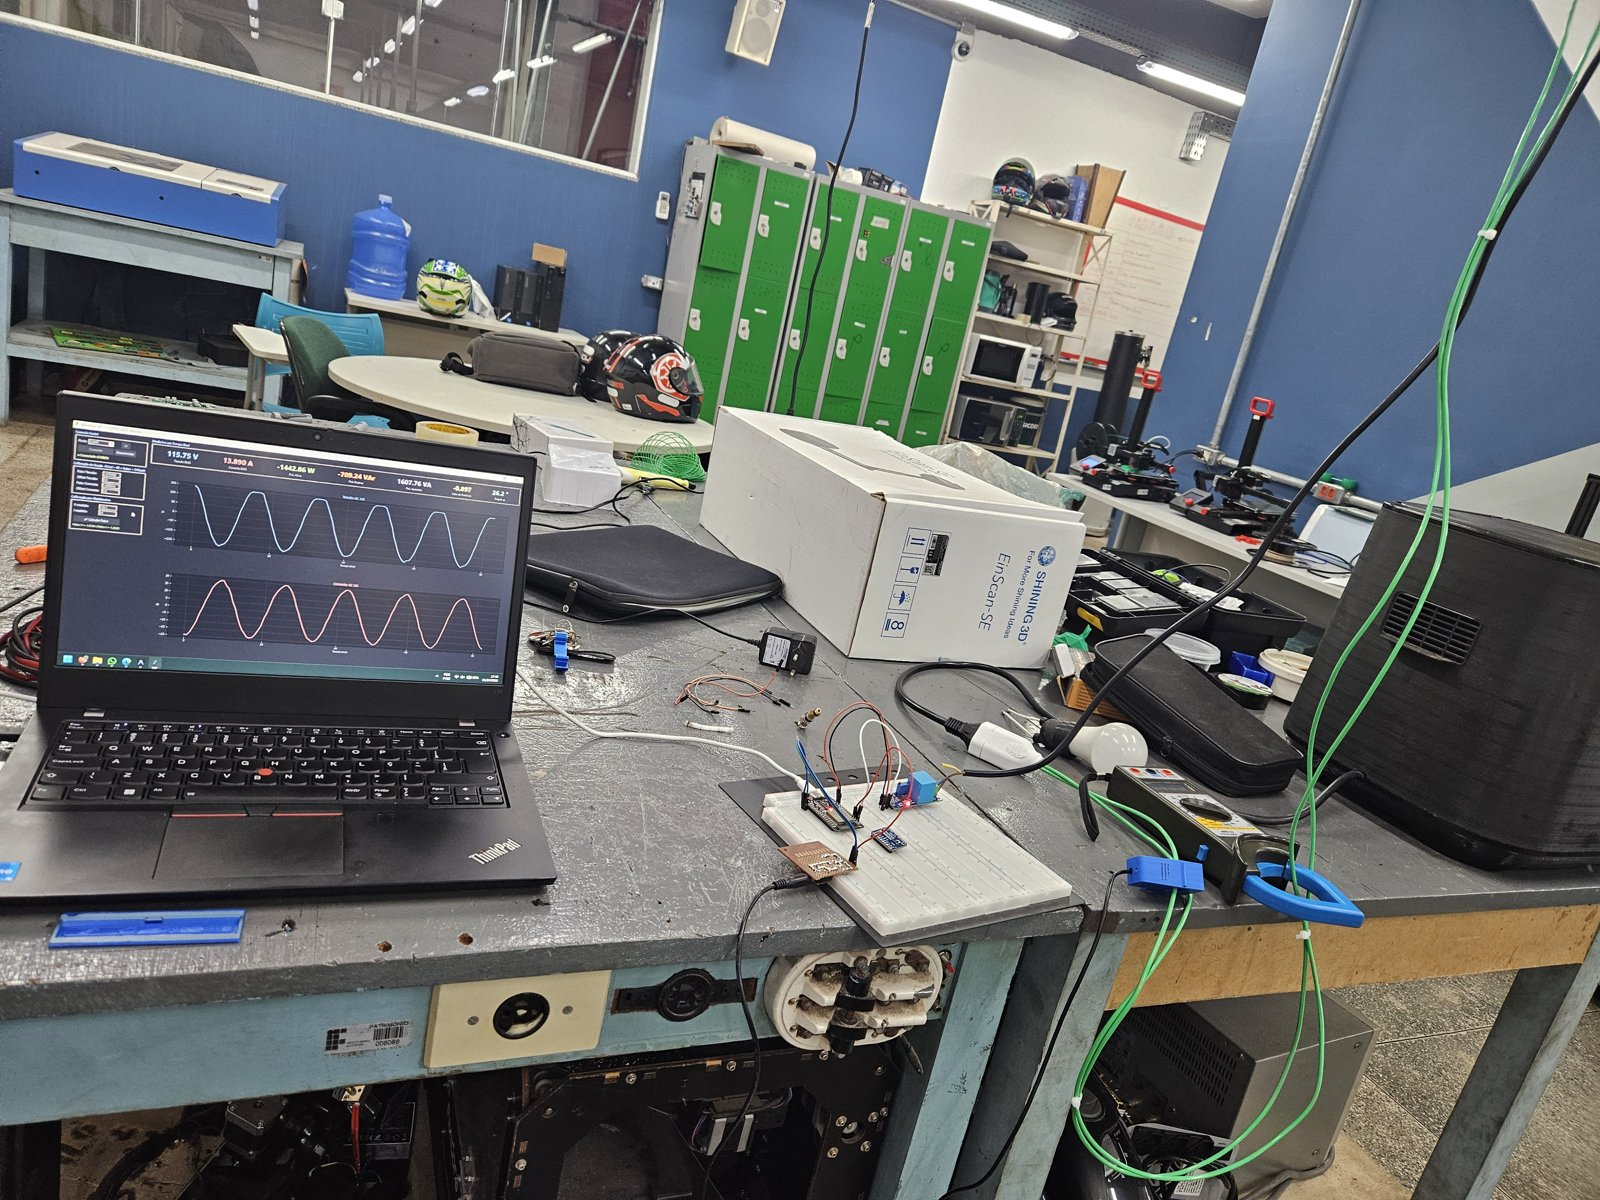
\includegraphics[width=\linewidth]{Testesimplificadoumafase.jpg}
    \caption{Teste simplificado da aquisi\c{c}\~ao em uma \'unica fase.}
    \label{fig:testeumafase}
  \end{minipage}\hfill
  \begin{minipage}{0.47\linewidth}
    \centering
    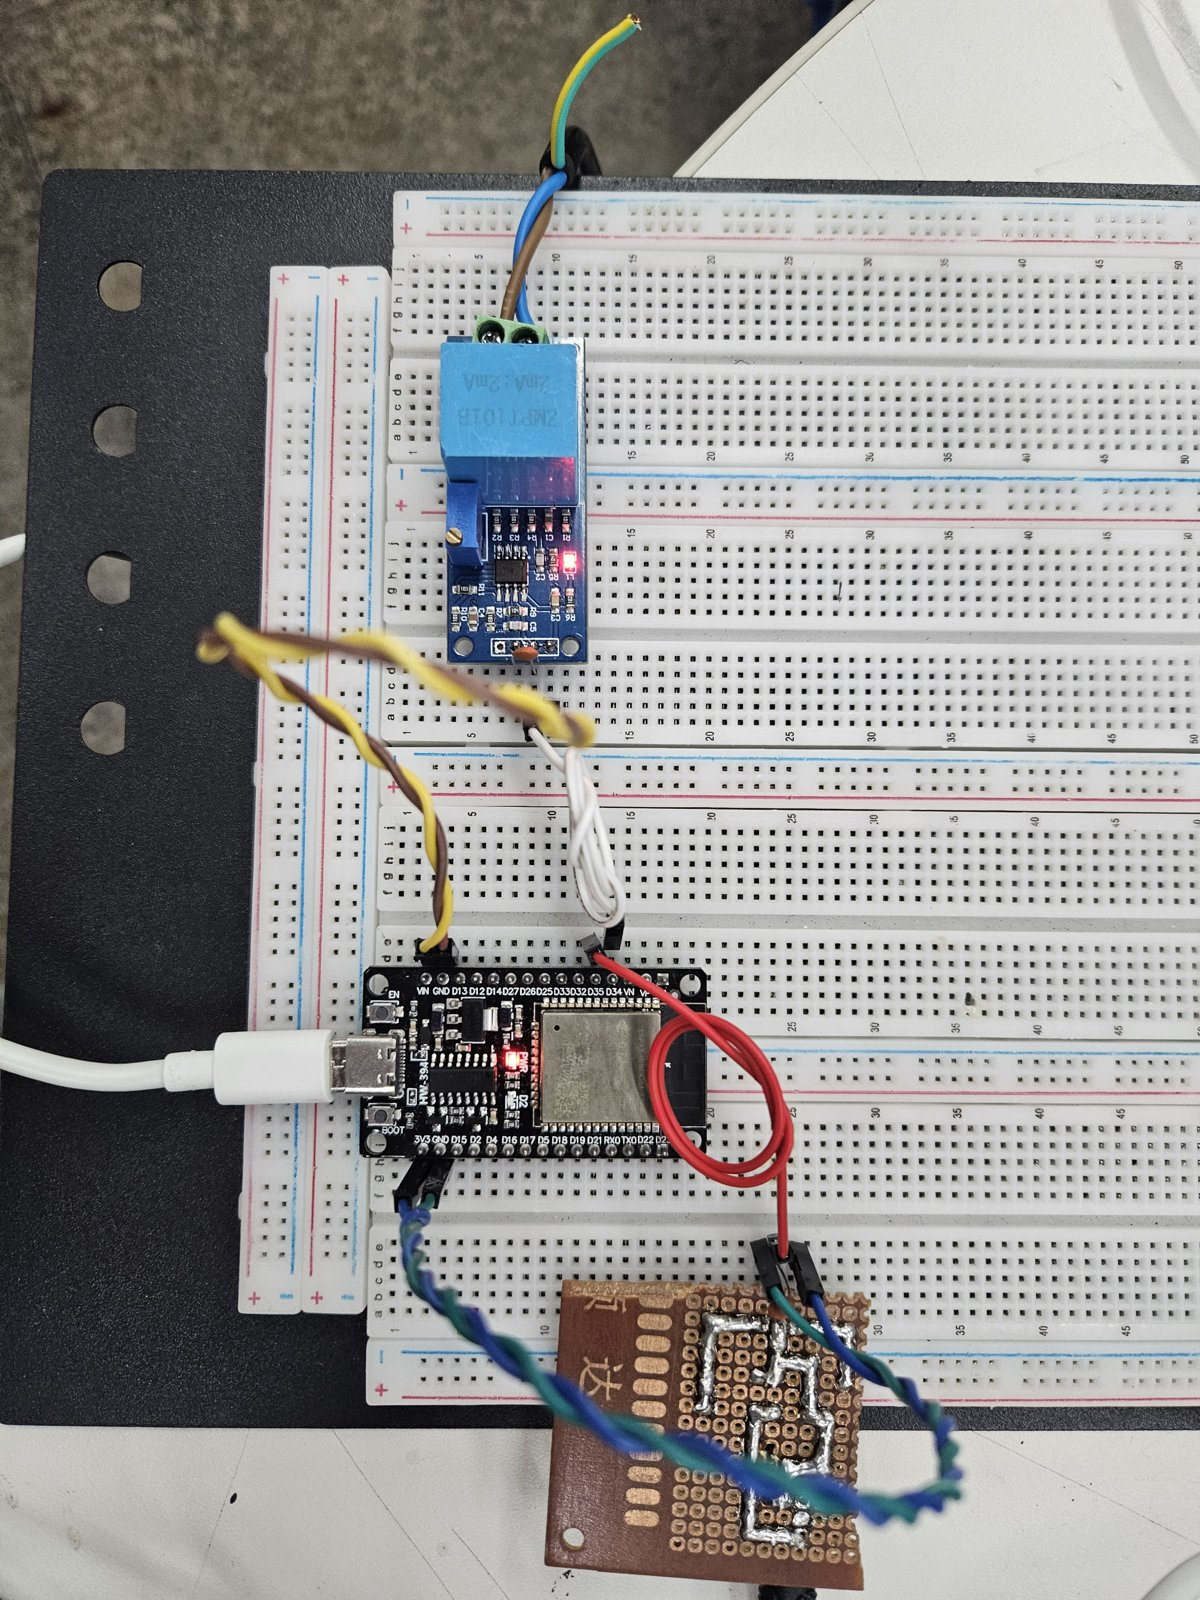
\includegraphics[width=\linewidth]{Prototipo1.jpg}
    \caption{Prot\'otipo em \textit{protoboard} com o sensor SCT-013 e m\'odulo ZMPT101B.}
    \label{fig:prototipo}
  \end{minipage}
\end{figure}
\FloatBarrier

\subsection{Sprint 2 -- \textit{Firmware} STM32, Telemetria e \textit{Dataset} (maio/2026)}
\begin{itemize}[nosep]
  \item \textbf{Objetivo:} consolidar a aquisi\c{c}\~ao bif\'asica de alta fidelidade
  no STM32 e montar a infraestrutura de transmiss\~ao e persist\^encia do
  \textit{dataset} (\'epico EP4).
  \item \textbf{Planejado:} \textit{firmware} STM32 e protocolo bin\'ario; monitor
  em Python; telemetria MQTT (US9); \textit{backend} de ingest\~ao (US10); tratamento
  de dados em CSV (US11); persist\^encia de kWh em LittleFS (US12).
  \item \textbf{Conclu\'ido:} c\'odigo de amostragem bif\'asico do STM32 e monitor
  PyQt5 exibindo formas de onda em tempo real (Figuras~\ref{fig:testesensores}
  e~\ref{fig:gui}); \textit{pipeline} MQTT do ESP-Network; \textit{broker} Mosquitto
  em servidor dedicado (192.168.1.80); \textit{logger} com coluna de fase, $|Q|$
  absoluto e rota\c{c}\~ao de esquema; instala\c{c}\~ao em painel el\'etrico real para
  coleta cont\'inua (Figuras~\ref{fig:painel1} e~\ref{fig:painel2}).
  \item \textbf{Dificuldades:} migra\c{c}\~ao das amostras de \texttt{int16} para
  \texttt{int32} (\textit{wrapping} em picos); \textit{overflow} do \textit{buffer}
  de recep\c{c}\~ao (256 vs.\ 1055 bytes/\textit{frame}); \textit{retain} MQTT
  indevido; regras de \textit{firewall} do servidor --- todos diagnosticados e
  corrigidos.
  \item \textbf{Entrega:} sistema bif\'asico com registro cont\'inuo resiliente,
  produzindo o \textit{dataset} que alimenta a Sprint~3.
\end{itemize}

\begin{figure}[ht]
  \centering
  \begin{minipage}{0.47\linewidth}
    \centering
    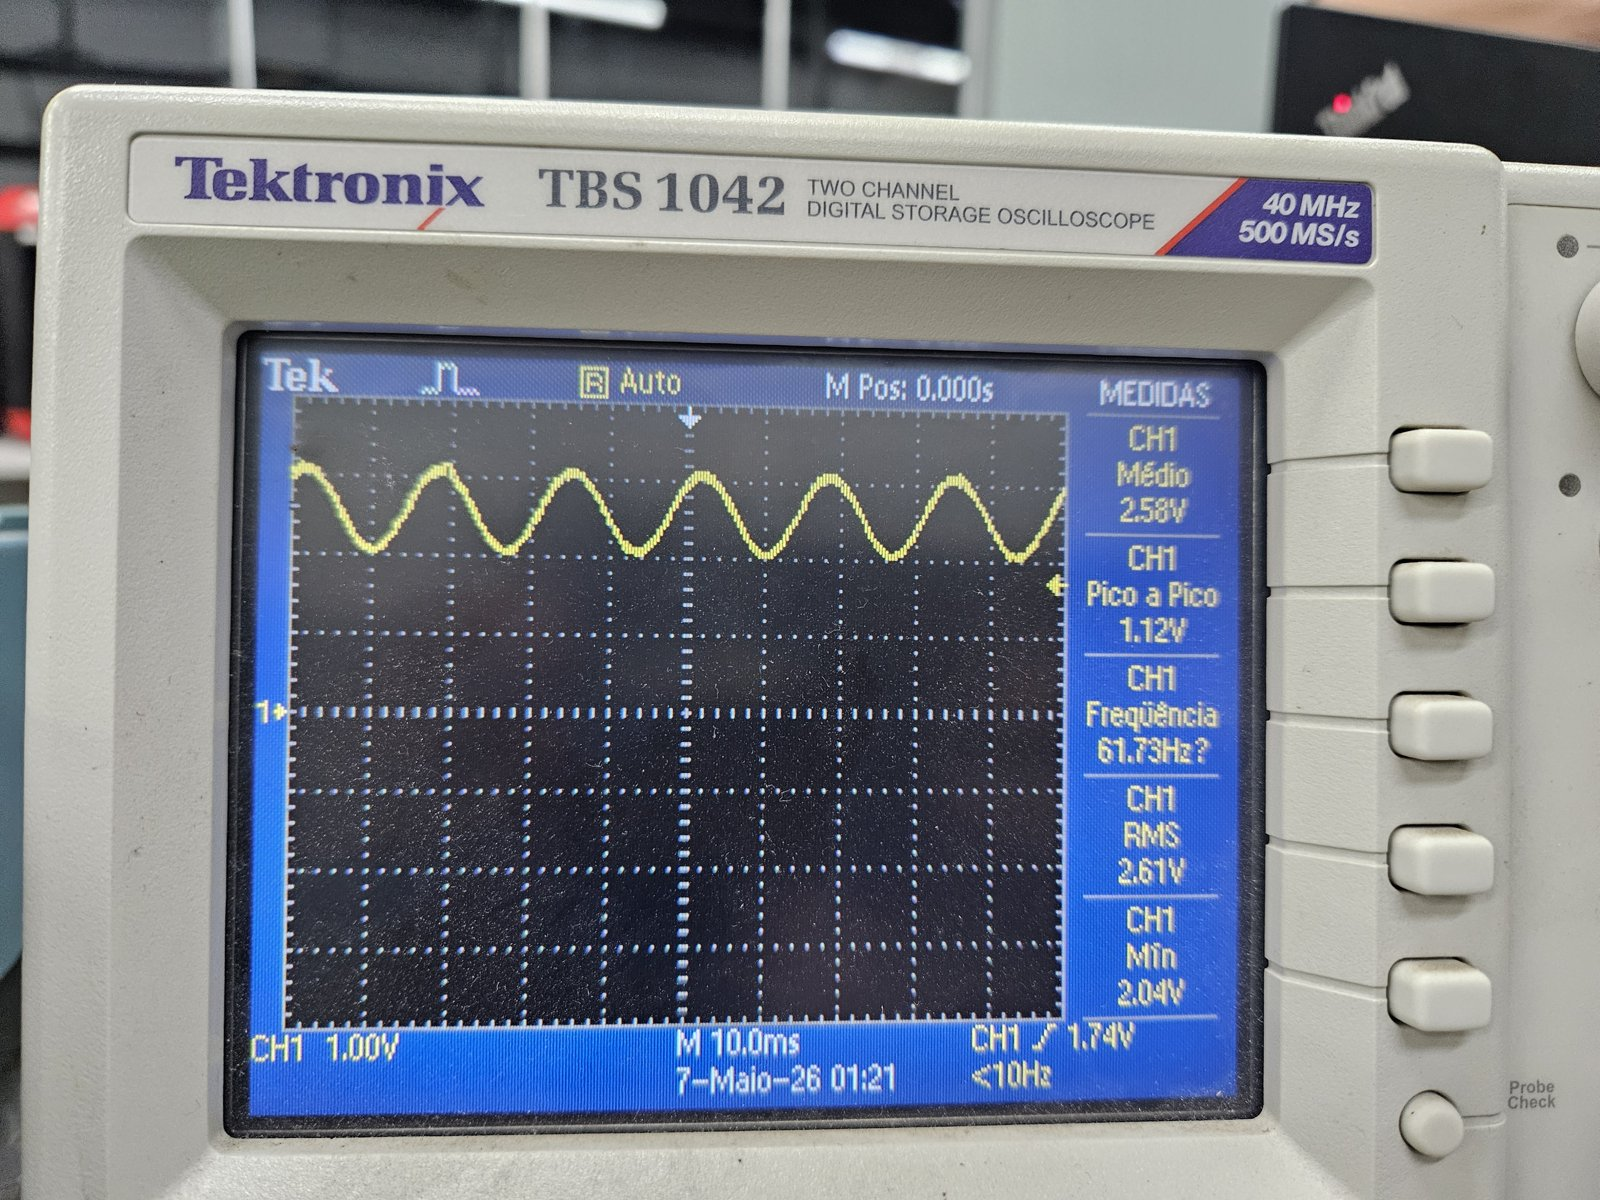
\includegraphics[width=\linewidth]{teste_sensores.jpg}
    \caption{Teste dos sensores de tens\~ao e corrente via oscilosc\'opio.}
    \label{fig:testesensores}
  \end{minipage}\hfill
  \begin{minipage}{0.47\linewidth}
    \centering
    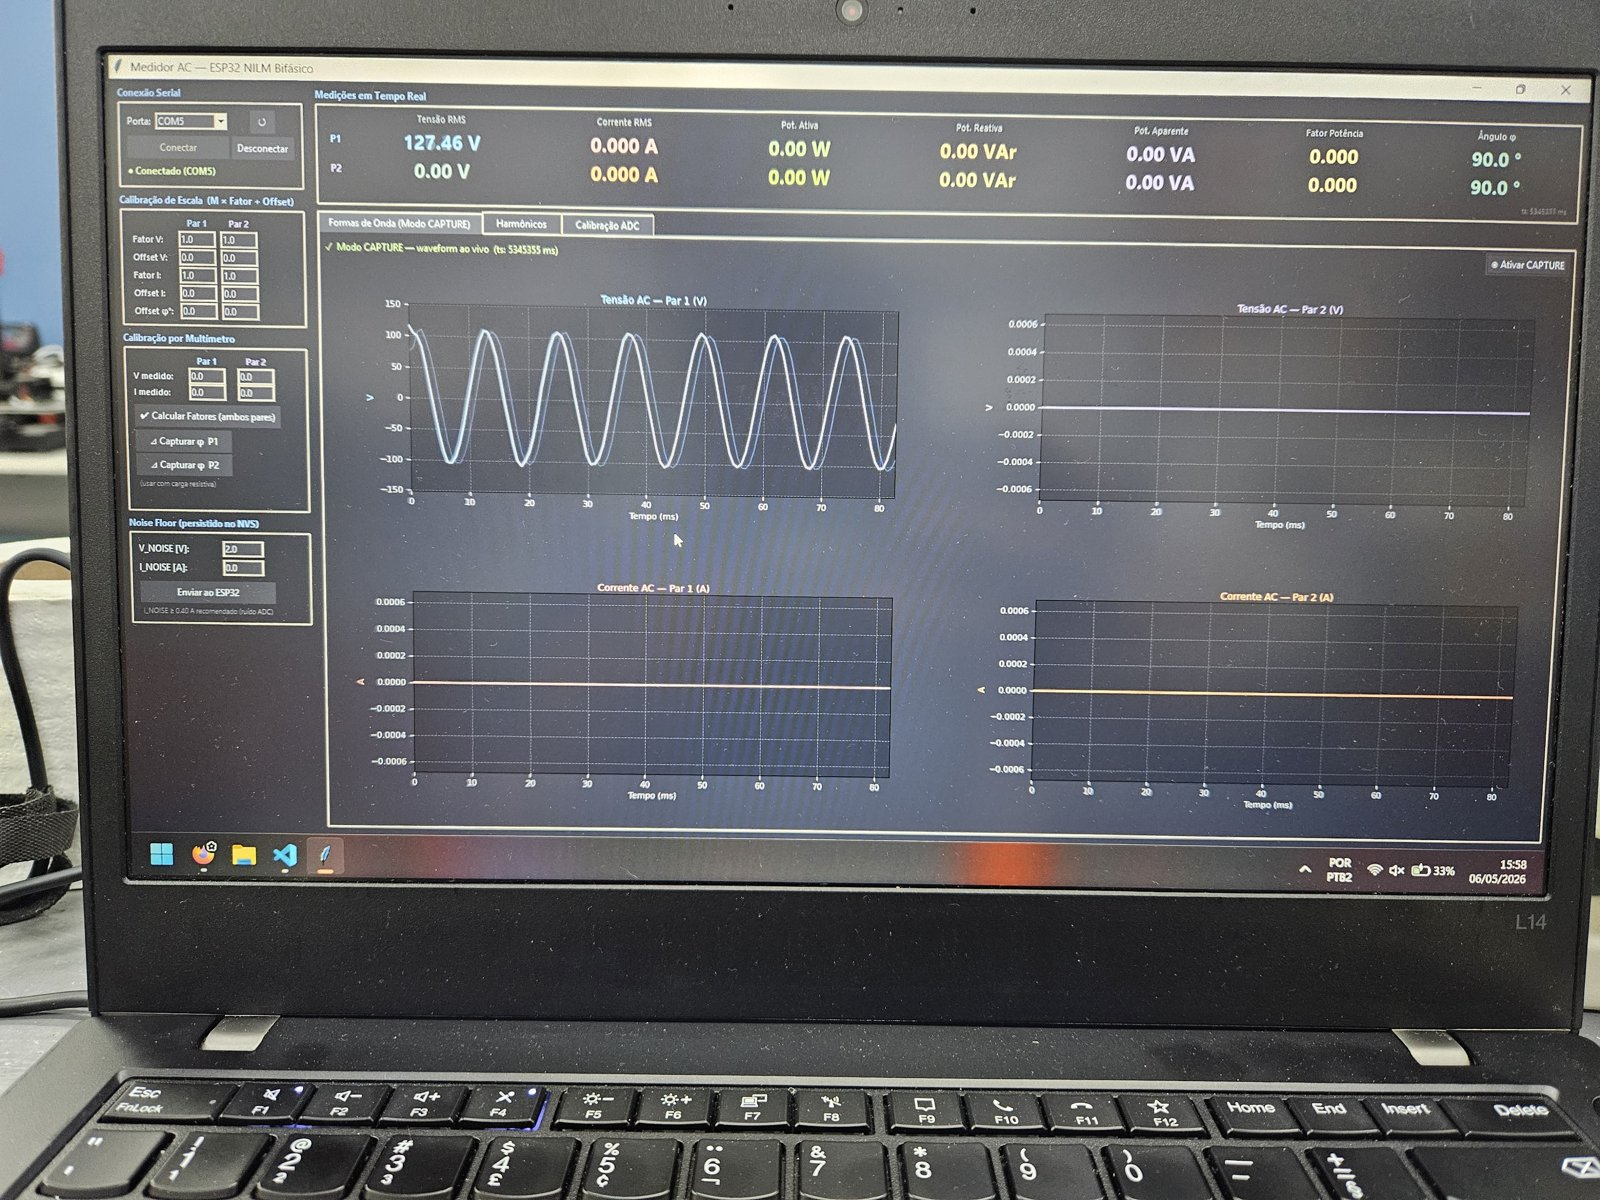
\includegraphics[width=\linewidth]{versaoInicialGUI.jpg}
    \caption{Vers\~ao inicial da interface de visualiza\c{c}\~ao (monitor Python).}
    \label{fig:gui}
  \end{minipage}
\end{figure}

\begin{figure}[ht]
  \centering
  \begin{minipage}{0.47\linewidth}
    \centering
    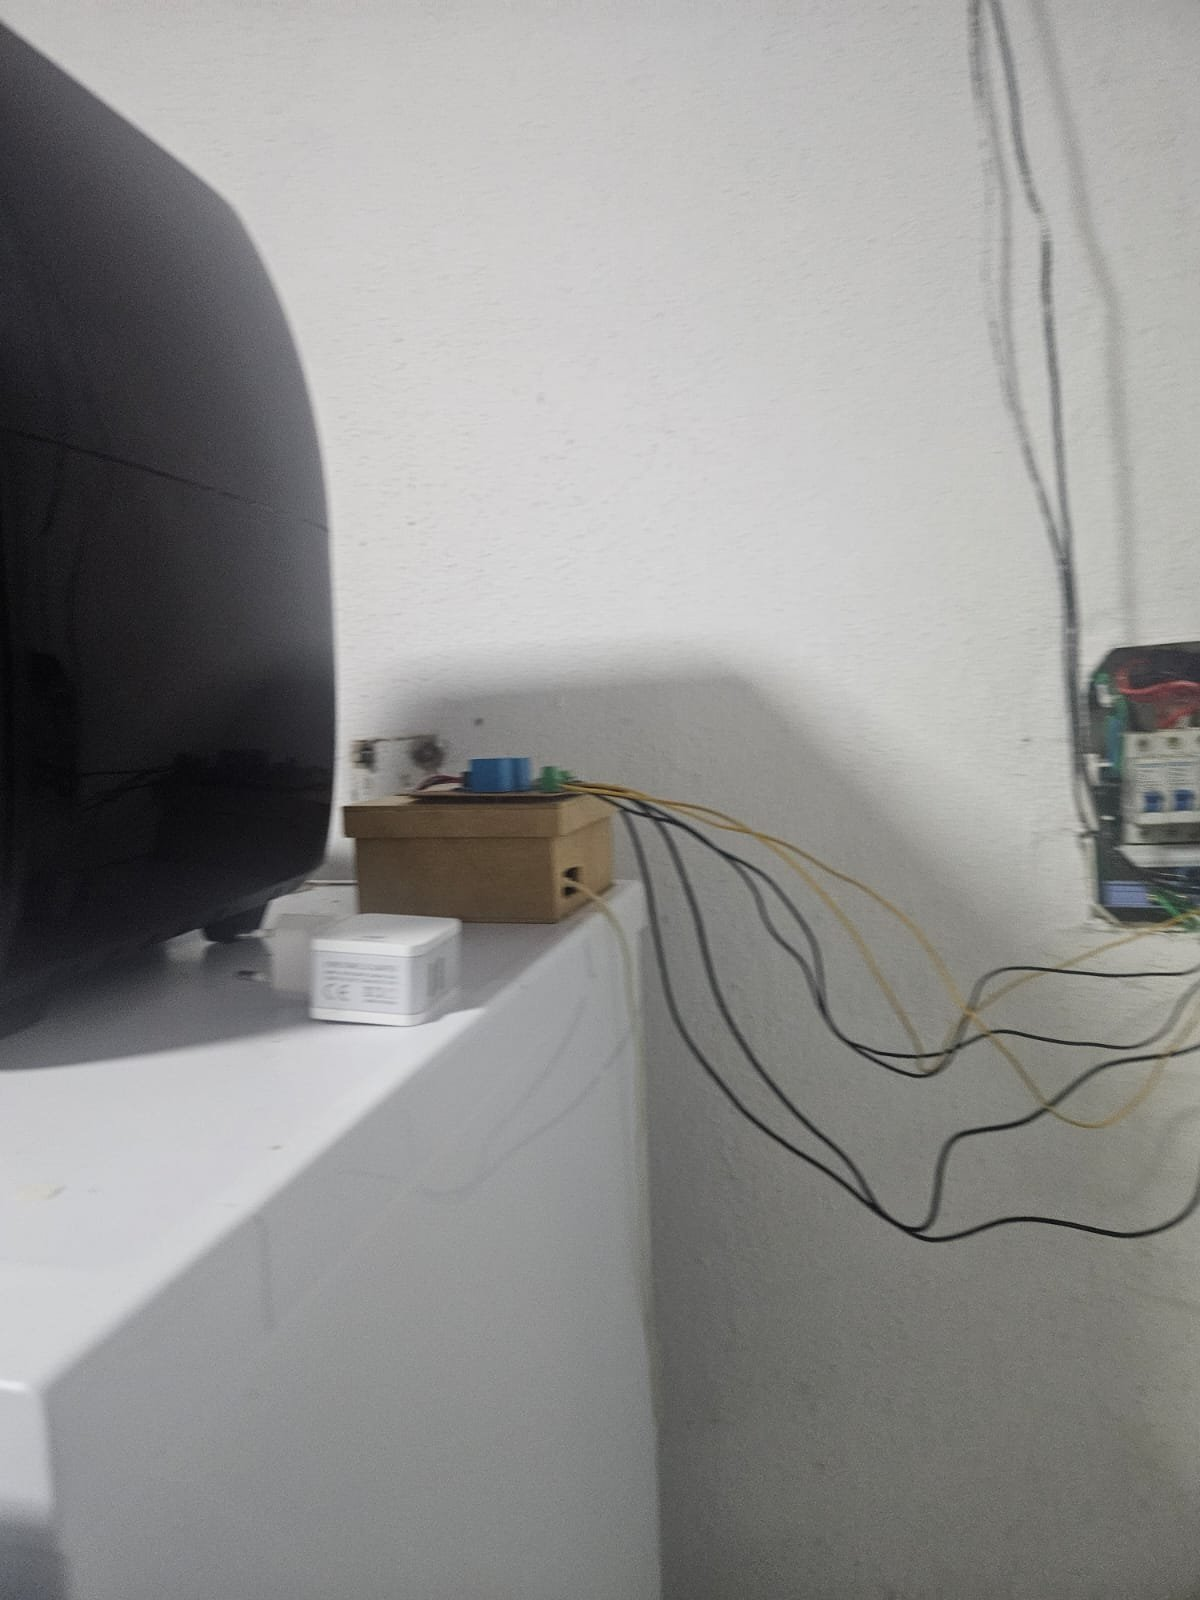
\includegraphics[width=\linewidth]{instalacaoPaineleletrico1.jpeg}
    \caption{Instala\c{c}\~ao do medidor no painel el\'etrico (vis\~ao geral).}
    \label{fig:painel1}
  \end{minipage}\hfill
  \begin{minipage}{0.47\linewidth}
    \centering
    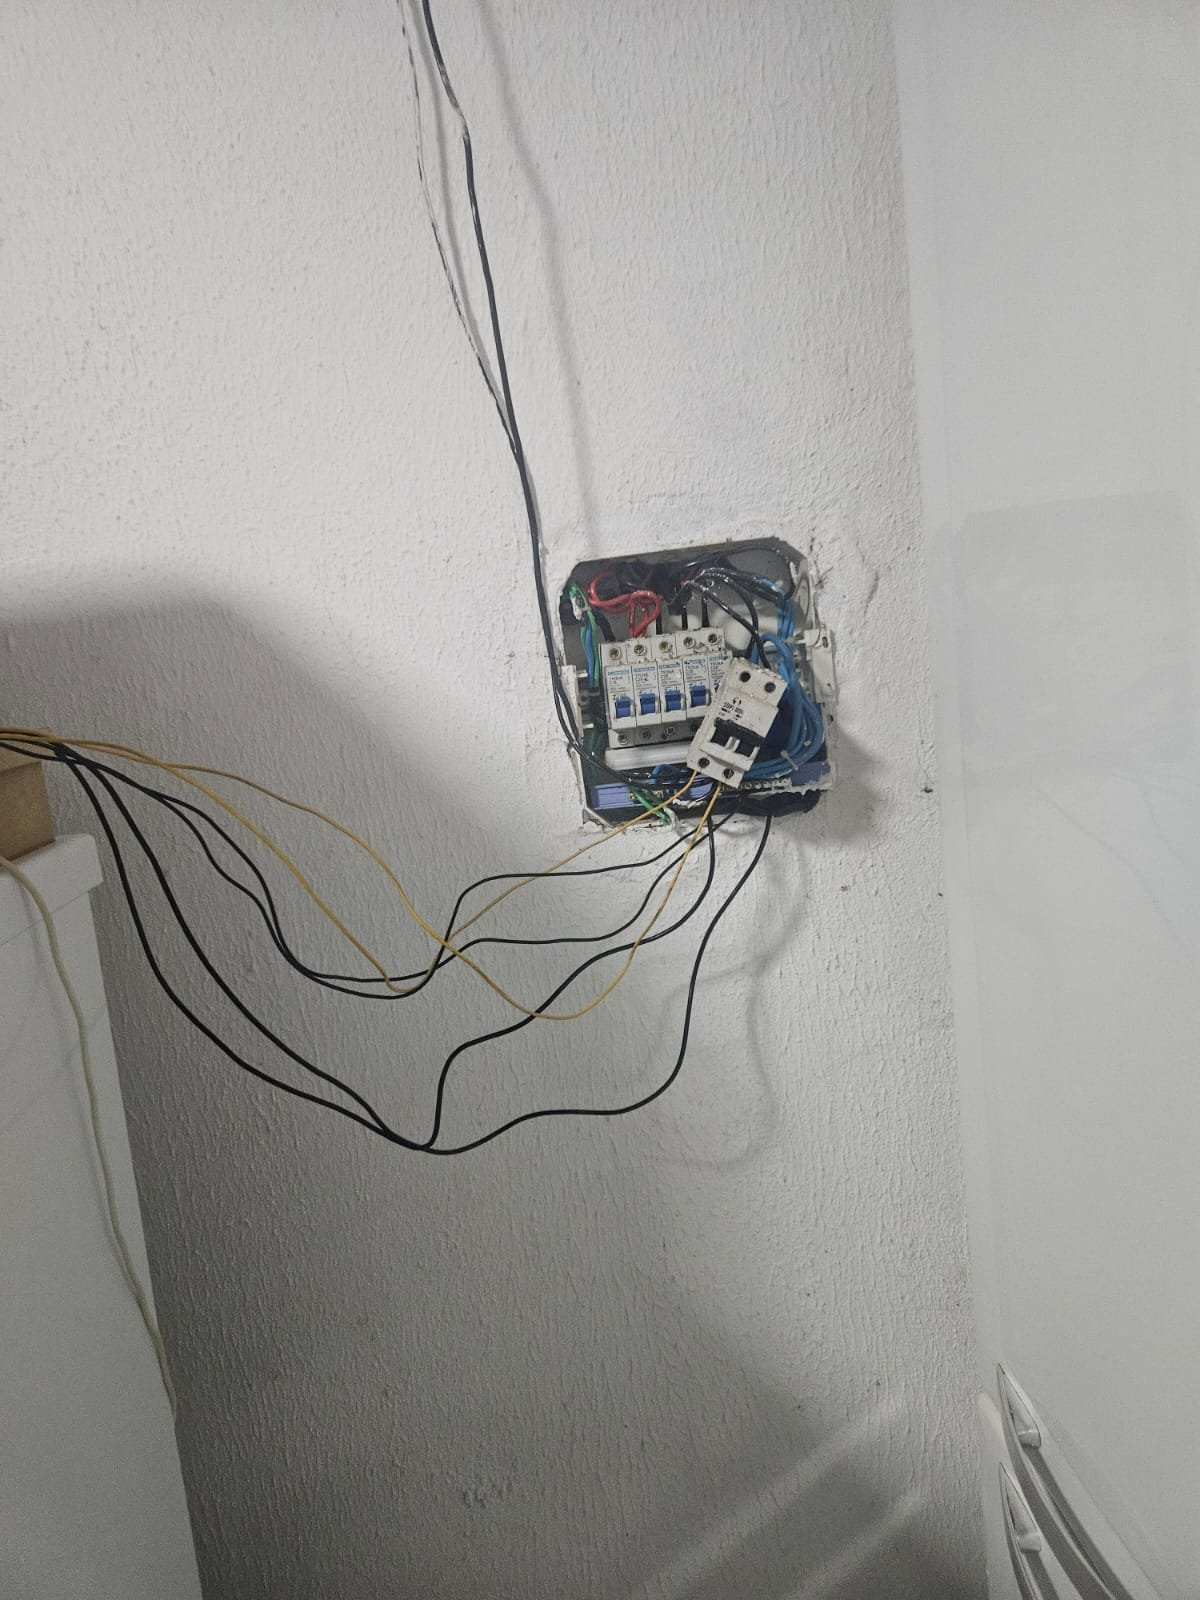
\includegraphics[width=\linewidth]{instalacaoPaineleletrico2.jpeg}
    \caption{Detalhe dos transformadores de corrente no painel.}
    \label{fig:painel2}
  \end{minipage}
\end{figure}
\FloatBarrier

\subsection{Sprint 3 -- Classifica\c{c}\~ao e Desagrega\c{c}\~ao (junho/2026)}
\begin{itemize}[nosep]
  \item \textbf{Objetivo:} desagregar as cargas a partir do \textit{dataset}
  coletado na Sprint~2 (\'epico EP3).
  \item \textbf{Planejado:} curadoria de \textit{dataset} rotulado (US6); modelagem
  de classifica\c{c}\~ao supervisionada (US7); estima\c{c}\~ao de consumo por
  infer\^encia cont\'inua (US8).
  \item \textbf{Conclu\'ido / desvio:} a curadoria de um \textit{dataset} rotulado
  (US6), pr\'e-requisito da classifica\c{c}\~ao supervisionada, mostrou-se invi\'avel
  em ambiente residencial n\~ao controlado (sem \textit{ground truth}). O \'epico
  foi \textbf{reorientado} para desagrega\c{c}\~ao \textbf{n\~ao supervisionada}:
  detector de eventos pr\'oprio, agrupamento K-means, teste de nulidade das
  caracter\'isticas harm\^onicas e valida\c{c}\~ao cruzada com o NILMTK (Hart85).
  Os resultados est\~ao detalhados na Se\c{c}\~ao~\ref{sec:resultados}.
  \item \textbf{Dificuldade:} dilui\c{c}\~ao dos \textit{clusters} pela massa de
  eventos de baixa pot\^encia.
  \item \textbf{Entrega:} \textit{pipeline} de desagrega\c{c}\~ao n\~ao supervisionada
  e o artigo t\'ecnico consolidando a metodologia e os resultados.
\end{itemize}
\FloatBarrier

\textbf{Funcionalidade n\~ao conclu\'ida.} A classifica\c{c}\~ao supervisionada com
m\'etricas quantitativas (F1-macro, matriz de confus\~ao --- \'epico EP3, US6--US8)
n\~ao foi finalizada, pois o ambiente n\~ao controlado n\~ao fornece
\textit{ground truth} (r\'otulos verdadeiros) das cargas. Em vez de abandonar o
\'epico, ele foi reorientado para a desagrega\c{c}\~ao n\~ao supervisionada, cujos
resultados est\~ao detalhados na Se\c{c}\~ao~\ref{sec:resultados}.

% ======================================================================
% 7. RESULTADOS
% ======================================================================
\section{Resultados Obtidos}
\label{sec:resultados}

\subsection{Produto Final}

O produto final \'e um medidor bif\'asico funcional que adquire, calcula, transmite
e persiste caracter\'isticas el\'etricas em opera\c{c}\~ao cont\'inua. As
Figuras~\ref{fig:funcional1} e~\ref{fig:funcional2} mostram o prot\'otipo funcional
montado, e a Figura~\ref{fig:fluxo} apresenta o fluxo de dados da arquitetura
\textit{Edge-to-Server}.

\begin{figure}[ht]
  \centering
  \begin{minipage}{0.47\linewidth}
    \centering
    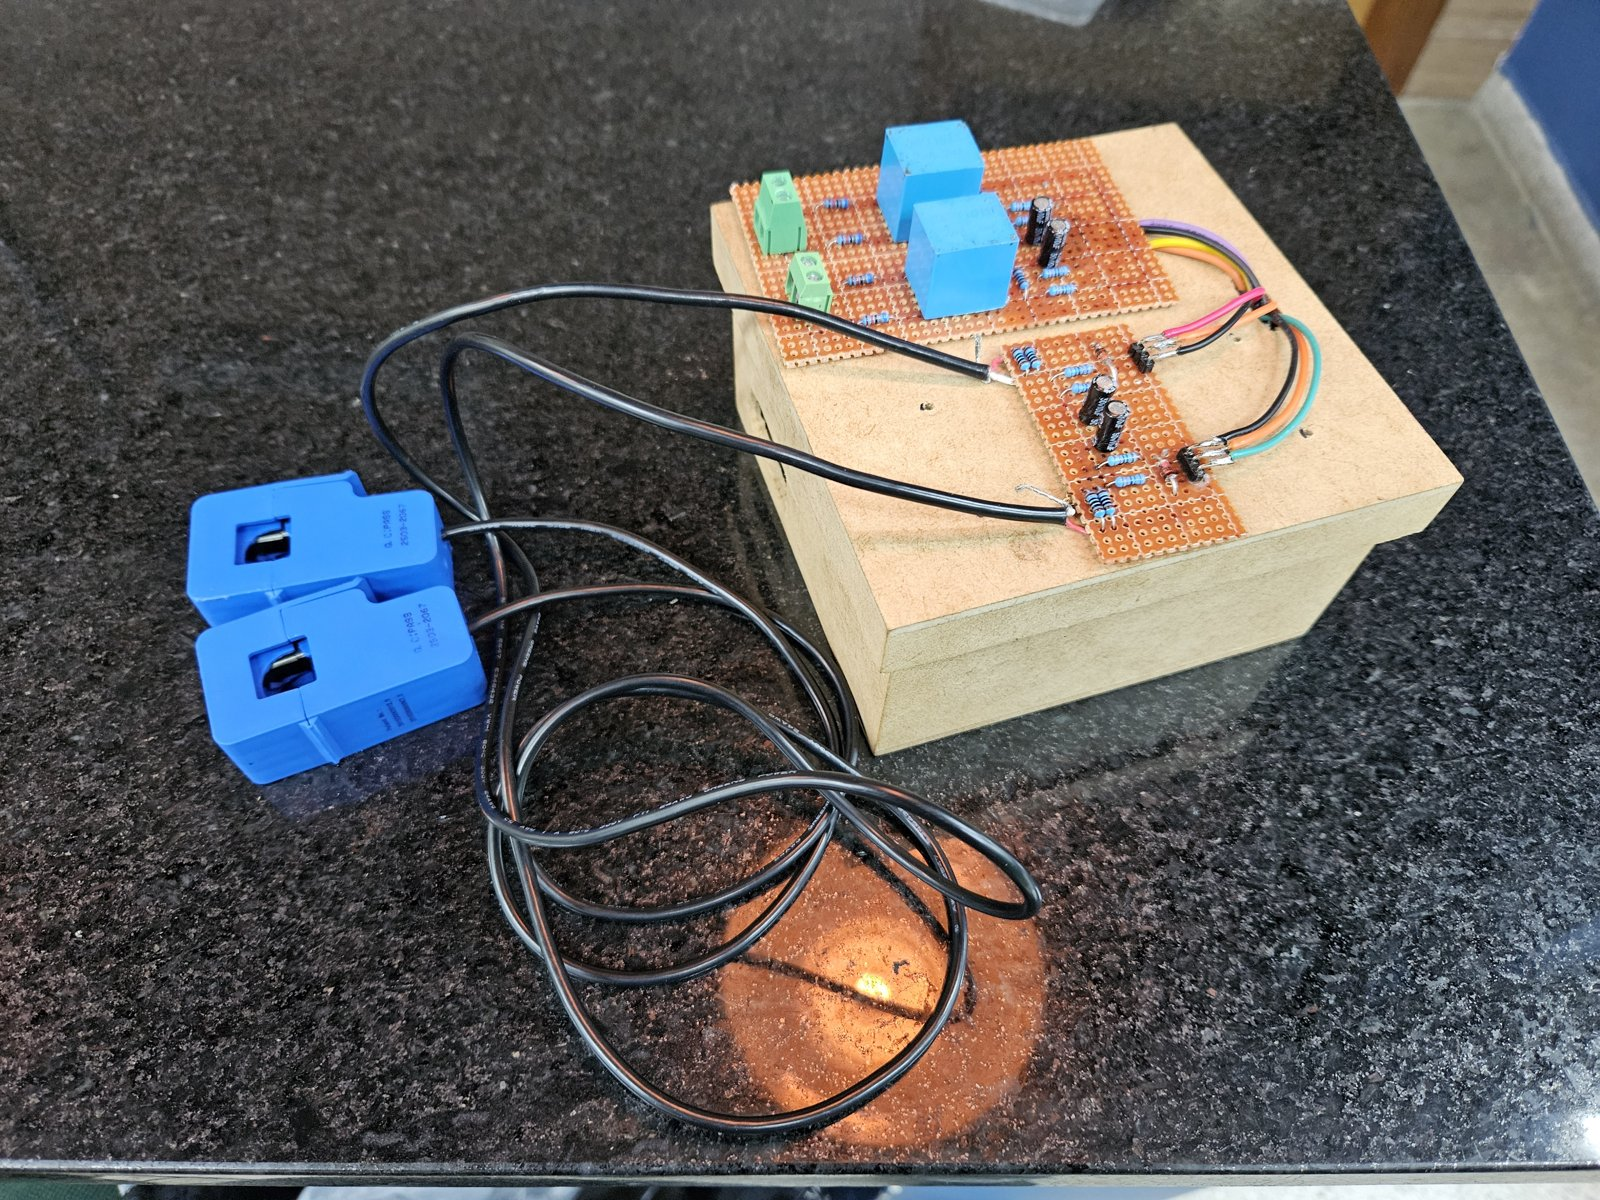
\includegraphics[width=\linewidth]{prototipofuncional1.jpg}
    \caption{Prot\'otipo funcional montado (vis\~ao geral).}
    \label{fig:funcional1}
  \end{minipage}\hfill
  \begin{minipage}{0.47\linewidth}
    \centering
    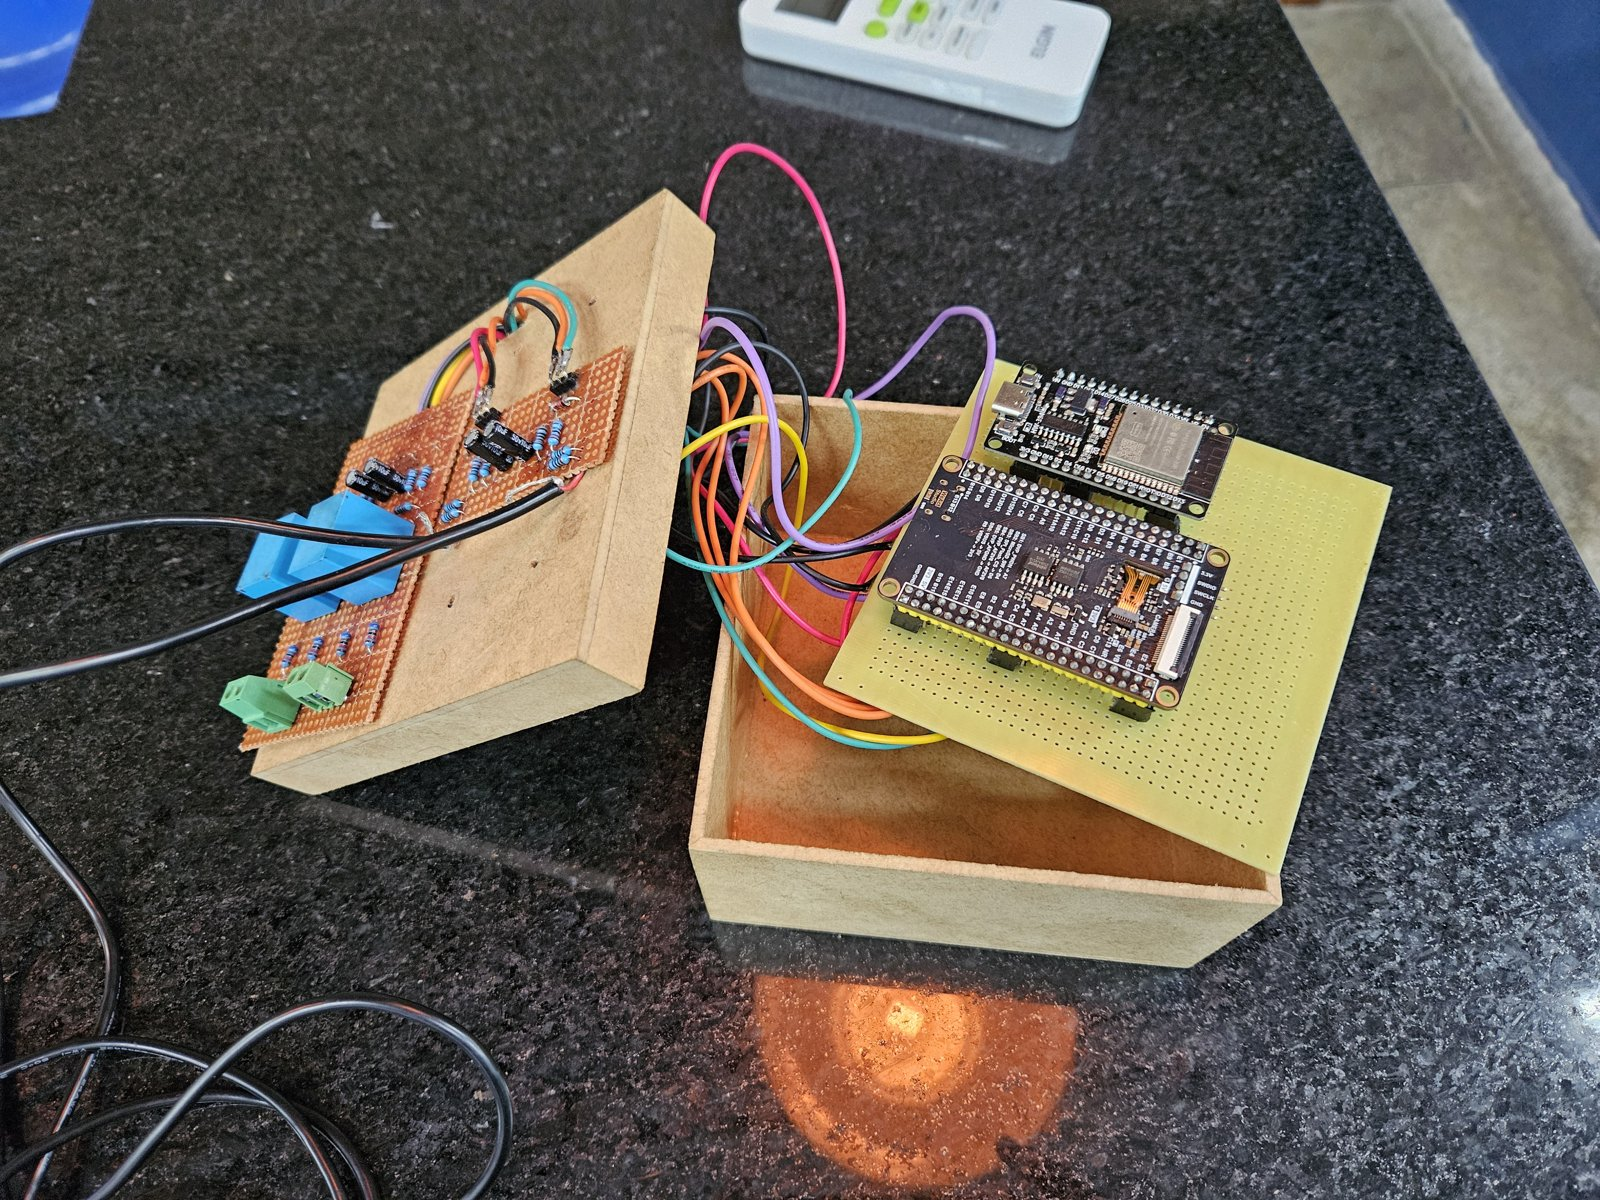
\includegraphics[width=\linewidth]{prototipofuncional2.jpg}
    \caption{Prot\'otipo funcional em opera\c{c}\~ao (detalhe).}
    \label{fig:funcional2}
  \end{minipage}
\end{figure}

\begin{figure}[ht]
  \centering
  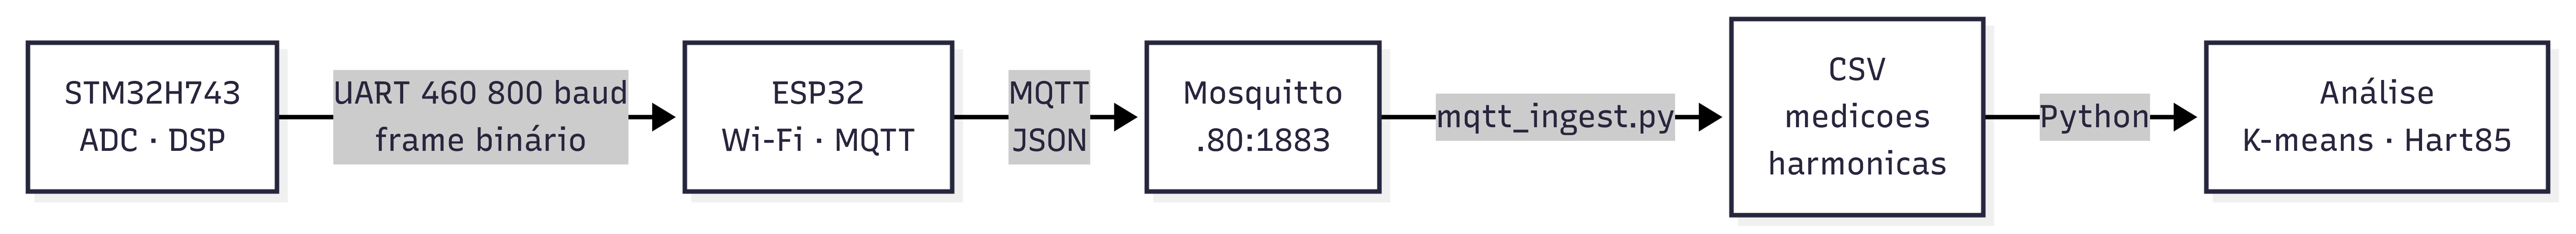
\includegraphics[width=0.95\linewidth]{fluxo-de-dados.png}
  \caption{Fluxo de dados: aquisi\c{c}\~ao no STM32H743, transmiss\~ao via ESP32/MQTT,
  ingest\~ao no servidor e an\'alise NILM.}
  \label{fig:fluxo}
\end{figure}
\FloatBarrier

\subsection{Funcionalidades Implementadas}

\begin{itemize}[nosep]
  \item Aquisi\c{c}\~ao bif\'asica simult\^anea a 15{.}360~Hz por fase, sem
  \textit{jitter}, via ADC/DMA sincronizados por temporizador.
  \item C\'alculo por ciclo de $V_{rms}$, $I_{rms}$, pot\^encia ativa, reativa e
  aparente, fator de pot\^encia e energia acumulada (kWh).
  \item C\'alculo do espectro harm\^onico (h1--h50) por Goertzel e da DHT de
  tens\~ao e corrente.
  \item Transmiss\~ao bin\'aria eficiente (\textasciitilde329~kbps sobre 460.800
  \textit{baud}) e publica\c{c}\~ao MQTT com \textit{throttle} por fase.
  \item Servidor de registro cont\'inuo (Mosquitto + \textit{logger}) com
  reinicializa\c{c}\~ao autom\'atica.
  \item \textit{Pipeline} de an\'alise NILM: detec\c{c}\~ao de eventos, agrupamento
  e teste de nulidade.
\end{itemize}

\subsection{Testes Realizados}

A cadeia de aquisi\c{c}\~ao foi validada com o monitor local (formas de onda e
espectro coerentes com tens\~ao nominal de 127~V e cargas reais). O detector de
eventos pr\'oprio foi confrontado com o algoritmo cl\'assico de Hart85 do
\textit{toolkit} NILMTK sobre os mesmos dados: a diverg\^encia no total de eventos
da Fase~2 ficou abaixo de 0{,}5\% (929 vs.\ 934), confirmando a corre\c{c}\~ao da
implementa\c{c}\~ao (Figura~\ref{fig:hart}).

\begin{figure}[ht]
  \centering
  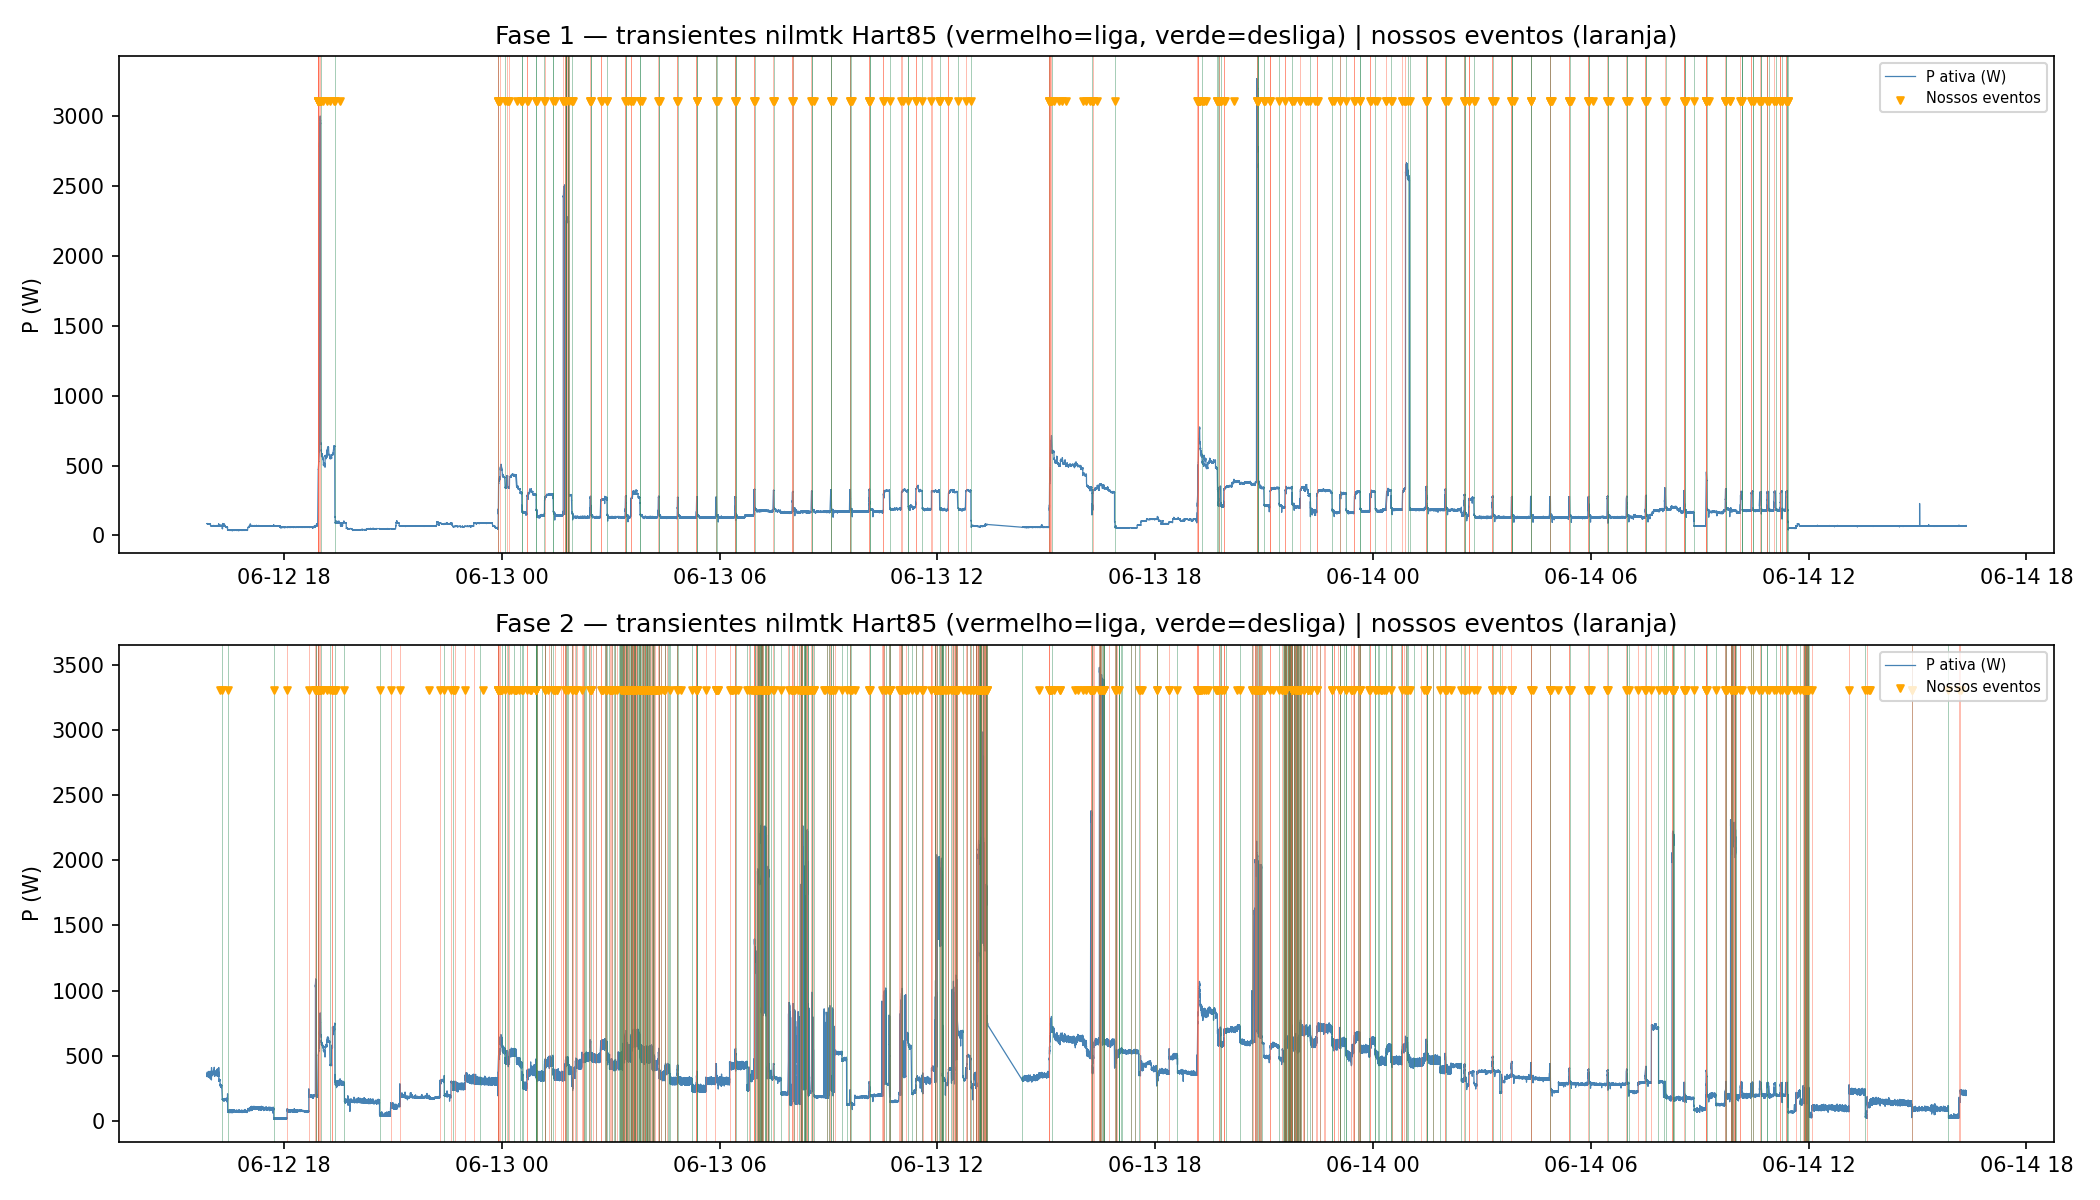
\includegraphics[width=\linewidth]{nilmtk_hart85_series.png}
  \caption{S\'erie de pot\^encia ativa com transientes detectados pelo Hart85
  (NILMTK). Vermelho = liga; verde = desliga. A base variável corresponde \`a
  modula\c{c}\~ao cont\'inua do compressor \textit{inverter}.}
  \label{fig:hart}
\end{figure}
\FloatBarrier

\subsection{Resultados da Desagrega\c{c}\~ao}

O agrupamento K-means sobre ($\Delta P$, $\Delta Q$) foi avaliado em janelas de
coleta crescentes. Com \textbf{um dia} de dados, o m\'etodo resolve aparentes 10
grupos, mas com baixa qualidade (silhueta 0{,}44 --- sobre-segmenta\c{c}\~ao). Com
\textbf{dois dias}, o n\'umero \'otimo de grupos colapsa para 3 (silhueta 0{,}74),
pois a massa de eventos de baixa pot\^encia passa a dominar
(Figura~\ref{fig:clusters}).

\begin{figure}[ht]
  \centering
  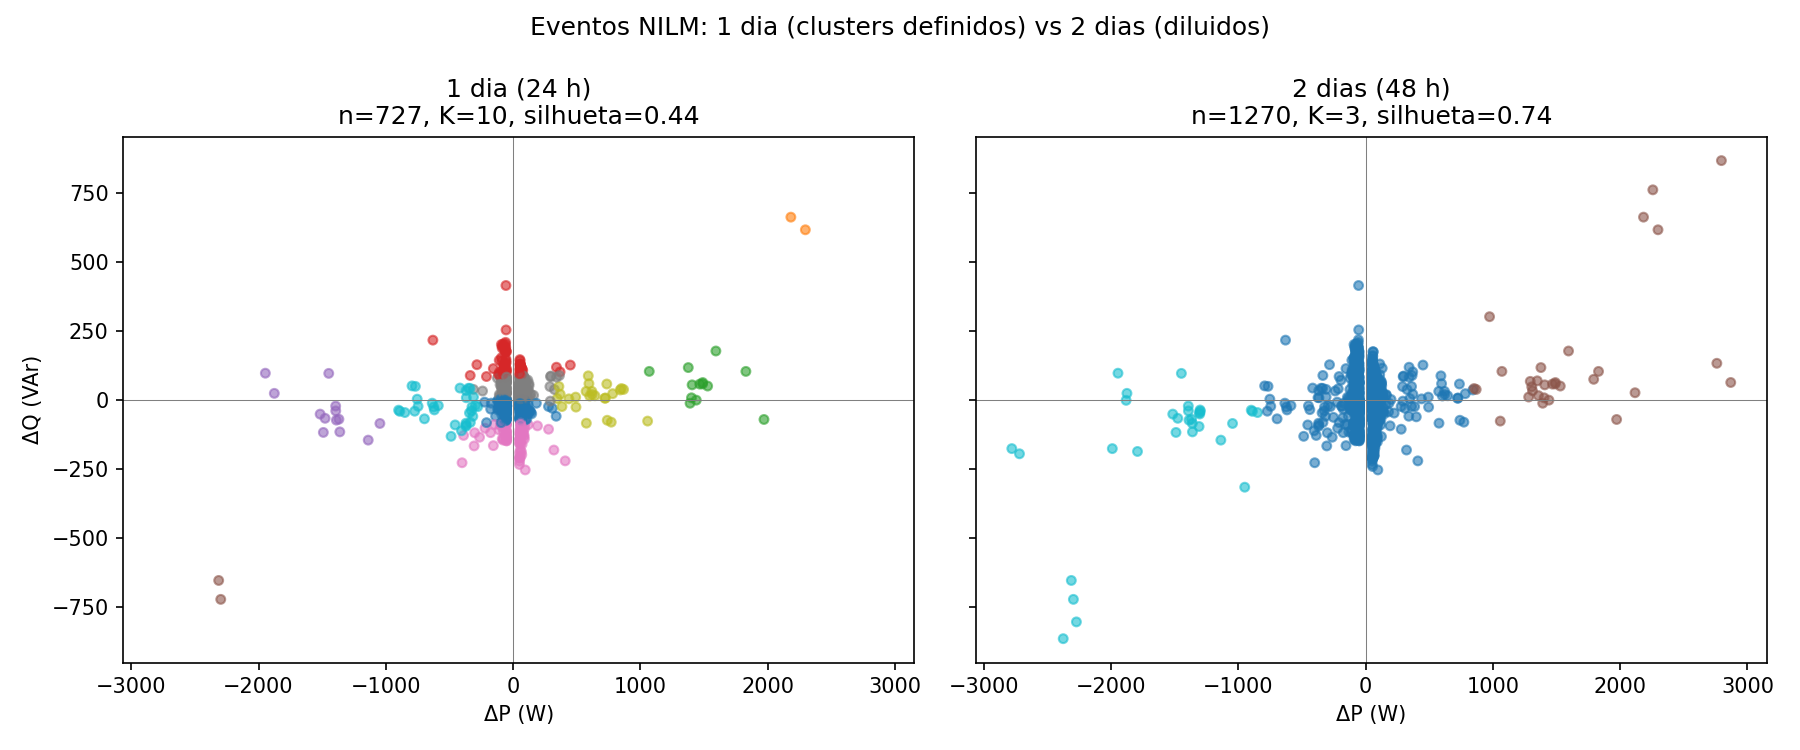
\includegraphics[width=\linewidth]{clusters_1d2d.png}
  \caption{Eventos no plano $\Delta P \times \Delta Q$: um dia (esquerda,
  sobre-segmenta\c{c}\~ao) \emph{vs.} dois dias (direita, agrupamento diluído).}
  \label{fig:clusters}
\end{figure}

A Figura~\ref{fig:degradacao} evidencia a degrada\c{c}\~ao da resolu\c{c}\~ao fina
\`a medida que os eventos de baixa pot\^encia se acumulam. Apenas as cargas de
maior pot\^encia (motor de $\approx$2{,}3~kW \emph{vs.}\ resistivas de
$\approx$800~W) permanecem separ\'aveis de forma est\'avel.

\begin{figure}[ht]
  \centering
  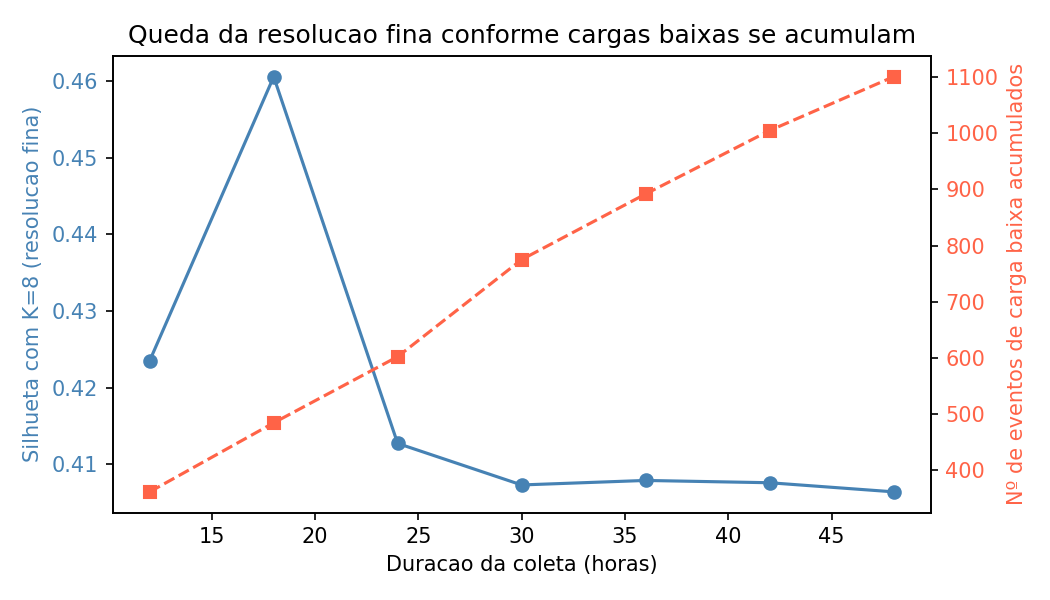
\includegraphics[width=0.8\linewidth]{degradacao.png}
  \caption{Queda da silhueta (resolu\c{c}\~ao fina, $K=8$) conforme os eventos de
  baixa pot\^encia se acumulam ao longo da coleta.}
  \label{fig:degradacao}
\end{figure}
\FloatBarrier

\textbf{Avalia\c{c}\~ao das caracter\'isticas harm\^onicas.} Um teste de nulidade
por permuta\c{c}\~ao (silhueta com harm\^onicos reais \emph{vs.}\ embaralhados)
demonstrou que os harm\^onicos \textbf{n\~ao agregam} informa\c{c}\~ao
discriminativa ao agrupamento neste \textit{setup} (Figura~\ref{fig:ablacao}): a
silhueta real coincide com a embaralhada. Trata-se de um resultado negativo
honesto e relevante, e n\~ao de uma falha.

\begin{figure}[ht]
  \centering
  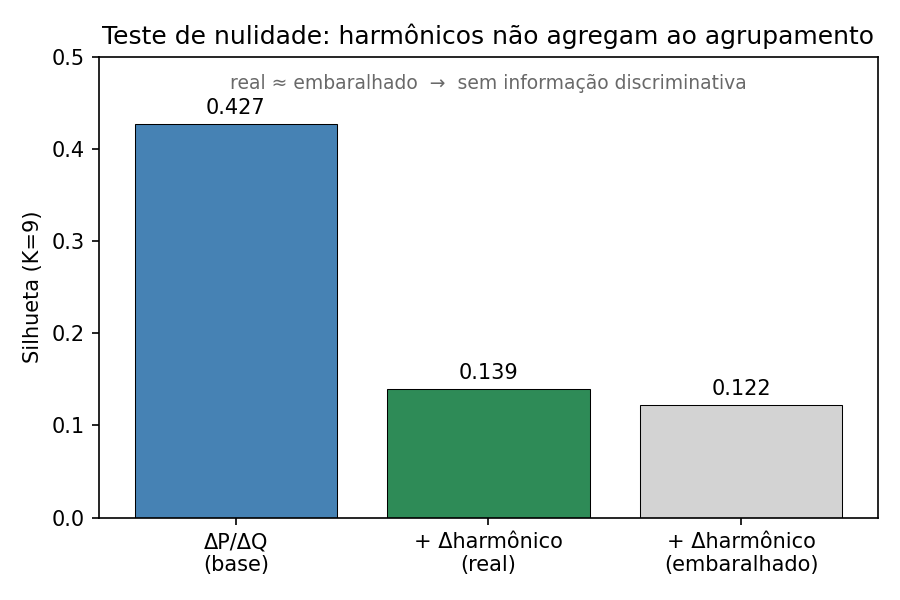
\includegraphics[width=0.7\linewidth]{ablacao_harmonicos.png}
  \caption{Teste de nulidade: a silhueta com $\Delta$harm\^onico real \'e
  estatisticamente igual \`a embaralhada e inferior \`a base $\Delta P$/$\Delta Q$.}
  \label{fig:ablacao}
\end{figure}
\FloatBarrier

\subsection{Benef\'icios Proporcionados}

O sistema entrega medi\c{c}\~ao de qualidade de energia (grandezas + harm\^onicos)
com \textit{hardware} de baixo custo relativo, tr\'afego de rede reduzido e
registro cont\'inuo --- uma base aberta e reprodut\'ivel para estudos de NILM.

\subsection{Limita\c{c}\~oes Identificadas}

\begin{itemize}[nosep]
  \item \textbf{Aus\^encia de \textit{ground truth}:} sem controle das cargas, a
  valida\c{c}\~ao quantitativa supervisionada (matriz de confus\~ao) fica
  comprometida; a avalia\c{c}\~ao recorre a m\'etricas internas (silhueta,
  estabilidade, plausibilidade f\'isica).
  \item \textbf{Cargas de modula\c{c}\~ao cont\'inua:} o compressor \textit{inverter}
  n\~ao produz degraus discretos e dilui os \textit{clusters}.
  \item \textbf{Sensoriamento:} n\~ao-linearidade do SCT-013 em baixa corrente e a
  taxa de amostragem efetiva mascaram transit\'orios de \textit{inrush}, \'uteis
  para distinguir cargas semelhantes.
\end{itemize}

\subsection{Reflex\~ao Final}

\textbf{Principais aprendizados.} A integra\c{c}\~ao \textit{hardware}--\textit{software}
em sistemas embarcados exige decis\~oes de engenharia criteriosas: o \textit{jitter}
do ESP32 e o \textit{overflow} de \textit{buffer} foram gargalos estruturais que
s\'o se revelaram em campo. No dom\'inio de dados, aprendeu-se o valor de um
\textbf{teste de nulidade} para separar estrutura real de artefato --- evitando
concluir, precipitadamente, que os harm\^onicos ajudariam.

\textbf{Dificuldades enfrentadas.} Est\'aveis: \textit{jitter} de amostragem,
\textit{overflow} de recep\c{c}\~ao serial, \textit{retain} MQTT indevido,
\textit{firewall} do servidor e a dilui\c{c}\~ao dos \textit{clusters} por cargas
de baixa pot\^encia.

\textbf{Melhorias futuras.} (i)~protocolo de aquisi\c{c}\~ao estruturado com
r\'otulos para viabilizar avalia\c{c}\~ao supervisionada; (ii)~captura de
transit\'orios de \textit{inrush} (\textit{trigger} de evento) para discriminar
cargas semelhantes; (iii)~conclus\~ao da migra\c{c}\~ao \texttt{int32} no
ESP-Network; (iv)~melhoria do condicionamento harm\^onico.

\textbf{Continuidade.} A plataforma est\'a documentada e versionada, apta a receber
novos algoritmos de desagrega\c{c}\~ao (incluindo modelos baseados em estados, como
FHMM) e a evoluir para um produto de monitoramento residencial.

% ======================================================================
% 8. ANEXOS
% ======================================================================
\section{Anexos}

\subsection{Link para o GitHub}

Reposit\'orio do projeto: \url{https://github.com/cmigos1/accuenergy}

\noindent O reposit\'orio cont\'em o c\'odigo-fonte atualizado (\textit{firmware}
STM32 e ESP32, monitor e \textit{scripts} de an\'alise), o hist\'orico completo de
\textit{commits} (24 \textit{commits}, mar--jun/2026), o \texttt{README.md} com
instru\c{c}\~oes de instala\c{c}\~ao/execu\c{c}\~ao e a documenta\c{c}\~ao t\'ecnica.

\subsection{Slides da Sprint Review}

Foi produzida a apresenta\c{c}\~ao de \textit{Sprint Review}
\texttt{AccuEnergy\_Sprint\_Review.pptx} (dispon\'ivel em \texttt{docs/slides/}),
utilizada na revis\~ao de sprint com o orientador para demonstrar a evolu\c{c}\~ao
do produto e as entregas realizadas. Por se tratar de projeto individual, apenas
uma revis\~ao foi formalizada em \textit{slides}; as demais foram conduzidas
diretamente, com o rastro das entregas preservado no hist\'orico de
\textit{commits} (Se\c{c}\~ao~6).

\subsection{Prints ou Fotos do Projeto}

A evolu\c{c}\~ao f\'isica do prot\'otipo est\'a documentada nas fotografias das
Sprints (Se\c{c}\~ao~6): o teste monof\'asico e o prot\'otipo em \textit{protoboard}
(Figuras~\ref{fig:testeumafase} e~\ref{fig:prototipo}), a bancada de sensores e a
interface inicial (Figuras~\ref{fig:testesensores} e~\ref{fig:gui}) e a
instala\c{c}\~ao no painel el\'etrico real (Figuras~\ref{fig:painel1}
e~\ref{fig:painel2}). O prot\'otipo funcional finalizado \'e mostrado nas
Figuras~\ref{fig:funcional1} e~\ref{fig:funcional2}. As figuras~\ref{fig:fluxo}
a~\ref{fig:ablacao} apresentam a
arquitetura de dados, a valida\c{c}\~ao da detec\c{c}\~ao de eventos e os resultados
da desagrega\c{c}\~ao.

\end{document}
